% ============================================================
%  Classificação Automática da Severidade da KOA — paper.tex
%  Compilar: latexmk -pdf paper.tex
% ============================================================
\documentclass[a4paper,12pt]{article}

% --- Codificação e idioma ---
\usepackage[utf8]{inputenc}
\usepackage[T1]{fontenc}
\usepackage[brazil]{babel}

% --- Tipografia e layout ---
\usepackage{microtype}
\usepackage[top=2.5cm,bottom=2.5cm,left=3cm,right=2.5cm]{geometry}
\usepackage{setspace}
\onehalfspacing

% --- Matemática ---
\usepackage{amsmath,amssymb,bm}

% --- Gráficos ---
\usepackage{graphicx}
\usepackage{float}
\usepackage{caption}
\usepackage{subcaption}
\graphicspath{{../data/output/figures/models/}{./}}

% --- Tabelas ---
\usepackage{booktabs}
\usepackage{multirow}
\usepackage{array}
\usepackage{tabularx}
\usepackage{adjustbox}
\usepackage{makecell}

% --- Código-fonte ---
\usepackage{listings}
\usepackage{xcolor}
\lstset{
  basicstyle=\ttfamily\footnotesize,
  breaklines=true,
  frame=single,
  backgroundcolor=\color{gray!10},
  numbers=none
}

% --- Hiperlinks e referências ---
\usepackage[numbers,sort&compress]{natbib}
\usepackage[hidelinks,colorlinks=true,
            linkcolor=black,citecolor=blue,urlcolor=blue]{hyperref}

% --- Utilitários ---
\usepackage{enumitem}
\usepackage{url}
\usepackage{lmodern}

% ============================================================
% Metadados
% ============================================================
\title{%
  \textbf{Classificação Automática da Severidade da Osteoartrite de Joelho
  a partir de Análise de Marcha 2D:}\\[4pt]
  \large Engenharia de \textit{Features} Biomecânicas e Ensemble LSTM com
  Validação Cruzada a Nível de Sujeito
}

\author{%
  Claudio Rank\thanks{Autor correspondente.}\\[2pt]
  \small Instituição / Departamento\\
  \small \texttt{clauciorank@gmail.com}
}

\date{\today}

% ============================================================
\begin{document}
% ============================================================
\maketitle
\thispagestyle{empty}

% ============================================================
\begin{abstract}
A osteoartrite de joelho (KOA) é uma das condições musculoesqueléticas
de maior prevalência global, responsável por substancial limitação funcional
e carga socioeconômica. A avaliação clínica convencional, baseada em radiografia
e escalas de graduação subjetivas, não captura alterações biomecânicas precoces
que antecedem a degeneração estrutural visível. Este trabalho propõe um pipeline
completo de classificação automática de KOA a partir de vídeos sagitais de marcha
2D, processados por estimativa de pose (OpenPose Body25), sem necessidade de
marcadores ou equipamentos especializados.

A abordagem combina 51 \textit{features} biomecânicas tabulares (parâmetros
espaço-temporais e cinemáticos articulares) com embeddings temporais extraídos
por um encoder LSTM (64 dimensões) em uma arquitetura ensemble com XGBoost.
Dois objetivos de classificação são avaliados: (Tarefa~A) triagem binária entre
controles normais (NM) e pacientes com KOA; e (Tarefa~B) estadiamento de
severidade em três graus (precoce, moderado e severo). A validação é conduzida
por validação cruzada estratificada de 5 \textit{folds} a nível de sujeito,
garantindo que nenhum participante integre simultaneamente os conjuntos de treino
e teste.

Os resultados demonstram que o XGBoost tabular atinge 94,7\%~$\pm$~3,4\% de
acurácia (F1 macro = 0,945; AUC = 0,994) na Tarefa~A, ao passo que o ensemble
XGB com encoder LSTM supera todos os modelos individuais na Tarefa~B, atingindo
79,6\%~$\pm$~6,4\% de acurácia (F1 macro = 0,804; AUC = 0,911), representando
uma melhora de 8,4 pontos percentuais sobre o XGBoost tabular isolado (71,2\%).
Adicionalmente, demonstramos que o encoder LSTM unidirecional (64 dimensões) iguala
ou supera o Bi-LSTM (128 dimensões) em ambas as tarefas, com metade da
dimensionalidade de embedding. Estes resultados superam o melhor resultado
comparável da literatura com protocolo equivalente de validação
(76,6\% de acurácia no estadiamento)~\cite{Kaya2025}.
\end{abstract}

\vspace{6pt}
\noindent\textbf{Palavras-chave:} osteoartrite de joelho; análise de marcha;
estimativa de pose; OpenPose; LSTM; ensemble; validação cruzada a nível de sujeito;
classificação biomecânica.

\newpage
\setcounter{page}{1}
\tableofcontents
\newpage

% ============================================================
\section{Introdução}
% ============================================================

A osteoartrite de joelho (KOA) constitui uma das principais causas de dor crônica
e incapacidade funcional na população adulta e idosa. Análises recentes do estudo
\textit{Global Burden of Disease} estimam que, em 2020, mais de 595 milhões de
pessoas viviam com osteoartrite em todo o mundo, com projeção de aumento de 74,9\%
nos casos de osteoartrite de joelho até 2050~\cite{GBD2023}. No Brasil, a
osteoartrite é a doença reumática mais prevalente, afetando mais de 15 milhões de
pessoas, com impacto direto na qualidade de vida e nos custos do sistema de saúde.

O diagnóstico e o monitoramento da KOA são fundamentados, na prática clínica, na
escala radiográfica de Kellgren-Lawrence (KL), que classifica a severidade em cinco
graus (0--4) com base em achados como estreitamento do espaço articular e formação de
osteófitos. Embora amplamente utilizada, essa escala apresenta limitações relevantes:
baixa sensibilidade para estágios iniciais, variabilidade inter-observador e ausência
de correlação direta com o estado funcional do paciente. Em estágios precoces
(KL~1--2), a estrutura articular pode estar preservada enquanto alterações
biomecânicas já estão presentes e causam sintomas.

A análise instrumental da marcha é reconhecida como biomarcador funcional sensível
para KOA. Pacientes com KOA apresentam redução da amplitude de movimento (ROM) do
joelho, encurtamento do comprimento de passo, aumento do tempo de apoio e maior
variabilidade intra-sujeito em comparação com controles saudáveis~\cite{Stenum2021,
Washabaugh2022}. Esses parâmetros podem ser extraídos de câmeras de vídeo
convencionais utilizando algoritmos de estimativa de pose, eliminando a necessidade
de sistemas de captura óptica com marcadores (custo elevado, restritos a laboratórios
especializados) ou sensores inerciais.

O OpenPose~\cite{Cao2021}, um dos algoritmos de estimativa de pose mais utilizados
em contextos clínicos, detecta automaticamente 25 \textit{keypoints} corporais em
vídeos monoculares com alta acurácia para cinemática de marcha no plano sagital:
erro médio de 5,1~$\pm$~2,5° para o joelho e 3,7~$\pm$~1,3° para o quadril,
comparado a sistemas de captura de movimento com
marcadores~\cite{Washabaugh2022}.

Apesar dos avanços recentes em aprendizado de máquina aplicado à análise de marcha,
a literatura apresenta uma lacuna metodológica importante: a maioria dos trabalhos
realiza a validação por \textit{random split} entre arquivos ou ciclos, sem
controlar o agrupamento de dados por sujeito. Essa prática introduz
\textit{data leakage} --- múltiplos ciclos do mesmo sujeito distribuídos entre
treino e teste ---, inflando artificialmente as métricas reportadas~\cite{Kaya2025}.
Apenas um trabalho recente~\cite{Kaya2025} adota explicitamente a validação a nível
de sujeito para o estadiamento de KOA, reportando queda de 14 pontos percentuais ao
migrar de \textit{random split} (90,8\%) para \textit{subject-based split} (76,6\%).

Este trabalho apresenta as seguintes contribuições:

\begin{enumerate}[label=\arabic*.]
  \item \textbf{Pipeline de análise completo e reproduzível:} da extração de poses
        com OpenPose Body25 à classificação por ensemble, com auditoria explícita de
        \textit{data leakage}.
  \item \textbf{Protocolo de validação rigoroso:} validação cruzada estratificada de
        5 \textit{folds} a nível de sujeito (\texttt{StratifiedGroupKFold}), sem
        vazamento de informação entre treino e teste.
  \item \textbf{Ensemble LSTM + tabular:} fusão explícita de embeddings temporais
        (64 dimensões) com \textit{features} biomecânicas tabulares (51 dimensões),
        obtendo +8,4 pp de melhora sobre XGBoost tabular no estadiamento de KOA.
  \item \textbf{Ablação experimental do encoder:} comparação sistemática entre
        encoder LSTM unidirecional e bidirecional (Bi-LSTM) com os mesmos
        hiperparâmetros e \textit{folds}, demonstrando que o LSTM iguala ou supera
        o Bi-LSTM com metade da dimensionalidade.
  \item \textbf{Melhor desempenho em estadiamento de KOA sob protocolo rigoroso:}
        79,6\% de acurácia vs.\ 76,6\% do melhor resultado comparável~\cite{Kaya2025}.
\end{enumerate}

% ============================================================
\section{Trabalhos Relacionados}
% ============================================================

\subsection{Estimativa de Pose para Análise de Marcha}

Stenum et al.~\cite{Stenum2021} demonstraram que o OpenPose pode extrair
automaticamente eventos de marcha (contato inicial e retirada do pé) e parâmetros
espaço-temporais a partir de vídeos 2D sagitais, com validade comparável a sistemas
com marcadores. O método de detecção de eventos baseado na posição relativa dos
tornozelos ao ponto médio do quadril (\textit{MidHip}) foi adotado integralmente neste
trabalho. Washabaugh et al.~\cite{Washabaugh2022} compararam múltiplos algoritmos de
estimativa de pose (OpenPose, MoveNet, MediaPipe) para mensuração de cinemática de
marcha, concluindo que o OpenPose apresenta o menor erro para ângulos do joelho
(5,1°~$\pm$~2,5°) e do quadril (3,7°~$\pm$~1,3°), sendo o mais adequado para
análise de marcha clínica 2D.

\subsection{Classificação de KOA por Análise de Marcha}

A Tabela~\ref{tab:comp} apresenta uma comparação sistemática dos trabalhos mais
recentes que utilizam o dataset público de Kour et al.~\cite{Kour2022} para
classificação de KOA.

\begin{table}[H]
  \centering
  \caption{Comparação com estudos que utilizam o mesmo dataset~\cite{Kour2022}.}
  \label{tab:comp}
  \small
  \begin{adjustbox}{max width=\textwidth}
  \begin{tabular}{@{}llll@{}}
    \toprule
    \textbf{Aspecto} &
    \textbf{Este estudo} &
    \textbf{Kaya et al.~\cite{Kaya2025}} &
    \textbf{Ben Hassine et al.~\cite{BenHassine2024}} \\
    \midrule
    Estimativa de pose &
      OpenPose Body25 (2D) &
      AlphaPose + HybrIK (3D) &
      Não especificado (2D) \\
    \textit{Features} &
      51 tabulares + LSTM &
      Ângulos 3D normalizados &
      Ângulos 2D + comprimento \\
    Melhor modelo &
      Ensemble XGB (LSTM enc.) &
      LSTM-FCN &
      Random Forest \\
    \textbf{Tarefa A --- NM vs.\ KOA} &
      \textbf{94,7\% (subj-CV)} &
      90,8\% (rand.) / 76,6\%$^\dagger$ &
      96,9\%$^\ddagger$ \\
    \textbf{Tarefa B --- KOA Staging} &
      \textbf{79,6\% (subj-CV)} &
      76,6\% (subj-CV) &
      --- \\
    Validação &
      5-fold subj-CV &
      5-fold (rand.\ + subj.) &
      Não reportada \\
    Auditoria de leakage &
      Sim (explícita) &
      Parcial &
      Não reportada \\
    Ablação de encoder &
      Sim (LSTM vs.\ Bi-LSTM) &
      Não &
      Não \\
    \bottomrule
  \end{tabular}
  \end{adjustbox}
  \vspace{4pt}

  {\footnotesize
  $^\dagger$ Kaya et al.~\cite{Kaya2025} reportam queda de 14,2 pp ao adotar
  \textit{split} por sujeito.\\
  $^\ddagger$ Protocolo de validação não detalhado em~\cite{BenHassine2024}.}
\end{table}

Kaya et al.~\cite{Kaya2025} utilizaram AlphaPose em combinação com HybrIK para
extrair ângulos articulares 3D e treinar um modelo LSTM-FCN, obtendo 76,6\% de
acurácia no estadiamento com validação por sujeito --- atualmente o resultado de
melhor referência para comparação direta. Ben Hassine et al.~\cite{BenHassine2024}
propuseram uma abordagem de Random Forest sobre \textit{features} extraídas de vídeos
2D, reportando 96,9\% na classificação binária NM vs.\ KOA, porém sem detalhar o
protocolo de validação.

\subsection{Justificativa para a Abordagem Ensemble}

A literatura em análise de marcha apoia o uso combinado de \textit{features}
biomecânicas interpretáveis com representações temporais aprendidas.
\textit{Features} tabulares como ROM, cadência e comprimento de passo capturam
padrões agregados, enquanto sequências temporais de ângulos articulares retêm
informações sobre padrões de movimento específicos da fase do ciclo que são
parcialmente perdidos na agregação~\cite{Stenum2021,Kaya2025}. A arquitetura
ensemble proposta neste trabalho explora essa complementaridade de forma explícita
e auditável.

% ============================================================
\section{Materiais e Métodos}
% ============================================================

\subsection{Conjunto de Dados}

Este trabalho utiliza o dataset público \textit{``A Vision-Based Gait Dataset for
Knee Osteoarthritis and Parkinson's Disease Analysis with Severity
Levels''}~\cite{Kour2022}, disponibilizado por Kour, Gupta e Arora (2022) na
plataforma Mendeley Data. O dataset contém gravações de vídeo sagital de marcha de
96 participantes distribuídos em três grupos: 30 controles saudáveis
(NM --- Normal), 50 pacientes com KOA (estadiados como precoce, moderado ou severo
segundo Kellgren-Lawrence) e 16 pacientes com doença de Parkinson (PD). O presente
estudo foca nas classes NM e KOA (Tabela~\ref{tab:dataset}); o grupo PD não foi
incluído nas análises e é discutido como extensão futura na Seção~\ref{sec:disc}.

\begin{table}[H]
  \centering
  \caption{Composição do dataset utilizado (grupos NM e KOA).}
  \label{tab:dataset}
  \begin{tabular}{@{}lrrrp{5.5cm}@{}}
    \toprule
    \textbf{Grupo} & \textbf{Sujeitos} & \textbf{Arquivos} &
    \textbf{Ciclos} & \textbf{Descrição} \\
    \midrule
    NM                & 30   & 60  & 324  & Controles saudáveis \\
    KOA-EL (Precoce)  & $\approx$17 & 28  & 248  & Estágio inicial (KL 1--2) \\
    KOA-MD (Moderado) & $\approx$19 & 38  & 345  & Estágio intermediário (KL 3) \\
    KOA-SV (Severo)   & $\approx$13 & 28  & 433  & Estágio avançado (KL 4) \\
    \midrule
    \textbf{Total Tarefa A} & \textbf{79} & \textbf{152} & \textbf{1350}
      & NM + todos KOA \\
    \textbf{Total Tarefa B} & \textbf{49} & \textbf{94} & \textbf{1026}
      & Apenas KOA (3 estágios) \\
    \bottomrule
  \end{tabular}
\end{table}

Os vídeos foram adquiridos com câmeras Logitech HD Pro C920 ou Nikon D5300 em
ambiente clínico controlado, com sujeitos caminhando no plano sagital a
1920~$\times$~1080~px a $\approx$50~fps. Cada sujeito realizou duas gravações
(sentido direita$\rightarrow$esquerda e esquerda$\rightarrow$direita).

\subsection{Estimativa de Pose}

A extração de \textit{keypoints} foi realizada com o modelo
\textbf{OpenPose Body25}~\cite{Cao2021} (modelo COCO com 25 \textit{keypoints},
versão 1.7.0), configurado com os parâmetros:

\begin{itemize}
  \item \texttt{number\_people\_max = 1} (vídeos com sujeito único);
  \item confiança mínima: 0,3 (conforme recomendação de Washabaugh et
        al.~\cite{Washabaugh2022});
  \item saída: $(T \times 25 \times 3)$ --- tempo $\times$ \textit{keypoints}
        $\times$ ($x$, $y$, confiança).
\end{itemize}

Dos 25 \textit{keypoints} do modelo Body25, 12 foram utilizados para a análise de
marcha: pescoço~(1), ponto médio do quadril~(8), quadril direito/esquerdo~(9/12),
joelho direito/esquerdo~(10/13), tornozelo direito/esquerdo~(11/14),
hálux direito/esquerdo~(22/19) e calcanhar direito/esquerdo~(24/21).

Os ângulos articulares no plano sagital foram calculados pelo produto interno entre
vetores segmentares:

\begin{equation}
  \theta_{\text{joelho}} =
  \arccos\!\left(\frac{\vec{u}_{\text{coxa}} \cdot \vec{u}_{\text{perna}}}
                      {|\vec{u}_{\text{coxa}}|\,|\vec{u}_{\text{perna}}|}\right)
  \label{eq:angle}
\end{equation}

\noindent onde $\vec{u}_{\text{coxa}} = \textit{quadril} - \textit{joelho}$ e
$\vec{u}_{\text{perna}} = \textit{tornozelo} - \textit{joelho}$.
Definições análogas foram aplicadas ao quadril (vetores tronco--quadril e
coxa--quadril) e ao tornozelo (vetores perna--tornozelo e hálux--tornozelo).

\subsection{Pré-processamento do Sinal}

O pipeline de pré-processamento foi implementado seguindo o protocolo de Stenum et
al.~\cite{Stenum2021}, com ajustes para o contexto de vídeo 2D
(Tabela~\ref{tab:preproc}).

\begin{table}[H]
  \centering
  \caption{Pipeline de pré-processamento.}
  \label{tab:preproc}
  \begin{tabular}{@{}llp{4.5cm}@{}}
    \toprule
    \textbf{Etapa} & \textbf{Método} & \textbf{Parâmetros} \\
    \midrule
    1.\ Mascaramento  & \textit{Keypoints} com conf.\ $<$ 0,3 $\rightarrow$ NaN
                      & Threshold: 0,3~\cite{Washabaugh2022} \\
    2.\ Interpolação  & Interpolação linear bidirecional
                      & Máximo: 5 frames ($\approx$100~ms) \\
    3.\ Suavização    & Filtro Butterworth zero-fase
                      & 4\textordfeminine\ ordem, corte 5~Hz \\
    4.\ Ângulos       & Produto interno entre vetores segmentares
                      & Plano sagital (2D) \\
    5.\ Eventos       & Posição relativa tornozelo/MidHip
                      & Heel Strike (HS) e Toe Off (TO)~\cite{Stenum2021} \\
    6.\ Ciclos        & Normalização HS$\rightarrow$HS (mesmo membro)
                      & 101 pontos via \textit{spline} cúbico \\
    7.\ QC            & Rejeição de ciclos com $>$ 20\% NaN
                      & Por articulação \\
    \bottomrule
  \end{tabular}
\end{table}

A detecção de eventos de marcha é baseada na posição horizontal relativa do
tornozelo ao ponto médio do quadril: o \textit{Heel Strike} corresponde ao máximo
local desta posição relativa (pé mais anterior), e o \textit{Toe Off} ao mínimo
local (pé mais posterior)~\cite{Stenum2021}. A validação fisiológica inclui
critérios de cadência (30--90 passos/min por membro) e tempo mínimo de passo
(300~ms). A normalização temporal de cada ciclo HS$\rightarrow$HS para 101 pontos
permite a comparação entre sujeitos com cadências distintas.

\subsection{Extração de \textit{Features}}

\subsubsection{\textit{Features} Tabulares (51 dimensões por arquivo)}

\textbf{Parâmetros espaço-temporais (8 \textit{features}):}
cadência (passos/min), tempo médio de passo (s), coeficiente de variação (CV) do
tempo de passo, comprimento médio de passo (pixels), CV do comprimento de passo,
tempo de apoio direito (s), tempo de apoio esquerdo (s) e índice de simetria (\%).

\textbf{Parâmetros cinemáticos articulares (42 \textit{features}):}
Para cada uma das 6 articulações (joelho direito/esquerdo, quadril direito/esquerdo,
tornozelo direito/esquerdo), foram calculadas 7 estatísticas sobre os ciclos
normalizados: ROM médio (°), desvio padrão (DP) do ROM, pico médio (°), DP do pico,
posição do pico (\% do ciclo), mínimo médio (°) e CV intra-ciclo (\%).

\textbf{Qualidade de detecção (1 \textit{feature}):}
Percentual médio de \textit{frames} válidos (confiança $\geq$ 0,3) nas articulações
de interesse (quadril, joelho, tornozelo), usado como covariável de qualidade.

\subsubsection{\textit{Features} Sequenciais ($101 \times 4$ por ciclo)}

Cada ciclo de marcha é representado como uma matriz $(101 \times 4)$, onde as colunas
correspondem aos ângulos normalizados de [joelho direito, joelho esquerdo, quadril
direito, quadril esquerdo] ao longo dos 101 pontos do ciclo normalizado. Ciclos com
mais de 20\% de valores ausentes foram descartados; NaNs residuais foram preenchidos
por interpolação \textit{forward}/\textit{backward}.

\subsection{Modelos de Classificação}

\subsubsection{Modelos Tabulares}

\textbf{XGBoost}~\cite{Chen2016}: \textit{gradient boosting} com 400 árvores,
profundidade máxima 5, taxa de aprendizado 0,05, \textit{subsample} 0,8 e
\textit{colsample\_bytree} 0,8. Objetivo \texttt{binary:logistic} (Tarefa~A) e
\texttt{multi:softprob} (Tarefa~B).

\textbf{Random Forest}~\cite{Breiman2001}: 500 árvores, sem profundidade máxima,
mínimo de 2 amostras por folha e \texttt{class\_weight=`balanced'}.

\textbf{SVM com \textit{kernel} RBF}~\cite{Cortes1995}: $C = 10$,
$\gamma = \texttt{scale}$, \texttt{class\_weight=`balanced'}. Todos os modelos
tabulares utilizam um \textit{pipeline} scikit-learn com \texttt{SimpleImputer}
(mediana) ajustado exclusivamente nos dados de treino de cada \textit{fold}.

\subsubsection{Modelos Sequenciais (LSTM e Bi-LSTM)}
\label{sec:lstm}

A arquitetura \textbf{GaitLSTM}~\cite{Hochreiter1997} recebe sequências de forma
$(B \times 101 \times 4)$ e utiliza:

\begin{lstlisting}
Entrada: (B, 101, 4)
 LSTM (hidden=64, layers=2, dropout=0.3)
 Ultimo timestep: (B, 64)
 Dropout (0.3)
 Linear: 64 -> num_classes
\end{lstlisting}

O \textbf{Bi-LSTM} é idêntico com \texttt{bidirectional=True}, resultando em
\textit{embedding} de 128 dimensões.

O treinamento utiliza otimizador Adam ($\eta = 10^{-3}$,
\textit{weight\_decay} $= 10^{-4}$), \textit{loss} \textit{CrossEntropy} com
pesos de classe inversamente proporcionais à frequência, gradiente limitado
(\textit{clip norm} $= 1{,}0$) e agendador \textit{ReduceLROnPlateau} (fator 0,5,
paciência 10 épocas). O modelo é treinado por \textbf{200 épocas fixas}
(sem \textit{early stopping}), com regularização via \textit{dropout} (0,3) e
\textit{weight decay} ($10^{-4}$). A calibração de 200 épocas foi confirmada
experimentalmente: a taxa de aprendizado convergiu para $3 \times 10^{-5}$ e o
ganho em acurácia nas últimas 10 épocas foi inferior a 0,4 pontos percentuais.

\subsection{Ensemble: Encoder LSTM + \textit{Features} Tabulares}
\label{sec:ensemble}

A arquitetura ensemble treina o encoder LSTM como extrator de representações
temporais dentro de cada \textit{fold}, concatena o \textit{embedding} resultante
com as \textit{features} tabulares e alimenta um classificador XGBoost (ou RF/SVM)
no espaço combinado.

\textbf{Pipeline do ensemble (por \textit{fold} de CV):}

\begin{enumerate}[label=\arabic*.]
  \item Treinar o encoder LSTM em todos os ciclos de treino do \textit{fold}
        (200 épocas).
  \item Extrair \textit{embeddings} do último \textit{timestep}:
        $\mathbf{e}_i \in \mathbb{R}^{64}$ por ciclo.
  \item Computar \textit{features} tabulares médias por sujeito:
        $\mathbf{t}_s \in \mathbb{R}^{51}$.
  \item Para cada ciclo $i$ do sujeito $s$:
        $\mathbf{x}_i = [\mathbf{e}_i \,\|\, \mathbf{t}_s] \in \mathbb{R}^{115}$.
  \item Treinar XGBoost em $\{(\mathbf{x}_i, y_i)\}$ de treino.
  \item Na inferência: predizer probabilidades por ciclo e agregar por sujeito
        (média).
\end{enumerate}

A \textbf{agregação ciclo$\rightarrow$sujeito} calcula a média das probabilidades de
todos os ciclos do sujeito e aplica argmax:

\begin{equation}
  \hat{y}_s = \arg\max_{c}\;
  \frac{1}{|C_s|} \sum_{i \in C_s} P\!\left(y = c \mid \mathbf{x}_i\right)
  \label{eq:agg}
\end{equation}

\noindent onde $C_s$ é o conjunto de ciclos do sujeito $s$. Esta abordagem garante
que a avaliação final seja equivalente à dos modelos tabulares (uma predição por
sujeito), tornando as comparações diretas e sem viés de granularidade.

O encoder é treinado integralmente dentro de cada \textit{fold}: os dados de teste
nunca são vistos durante o treinamento do LSTM nem durante o ajuste do XGBoost. A
\textit{feature} tabular média por sujeito ($\mathbf{t}_s$) é calculada sobre todos
os sujeitos, mas como é uma função determinística dos dados sem parâmetros
ajustáveis, não constitui fonte de leakage.

\subsection{Protocolo de Validação}

A validação adota \textbf{validação cruzada estratificada de 5 \textit{folds} a nível
de sujeito} (\texttt{StratifiedGroupKFold}, scikit-learn), com:

\begin{itemize}
  \item Chave de agrupamento: \texttt{"\{GRUPO\}\_\{ESTÁGIO\}\_\{ID\}"}
        (p.ex.\ \texttt{KOA\_EL\_001}), garantindo que sujeitos com mesmo ID
        numérico, mas estágios distintos, sejam tratados como participantes
        independentes.
  \item Estratificação por classe para manter proporções aproximadas em cada
        \textit{fold}.
  \item \textit{Seed} fixo (42) para reprodutibilidade.
  \item Tarefa~A: $\approx$63 sujeitos de treino / $\approx$16 de teste por
        \textit{fold}.
  \item Tarefa~B: $\approx$39 sujeitos de treino / $\approx$10 de teste por
        \textit{fold}.
\end{itemize}

Nenhum sujeito aparece simultaneamente nos conjuntos de treino e teste. As métricas
reportadas são médias e desvios padrão entre os 5 \textit{folds}.

As métricas utilizadas são: acurácia, F1 macro (média não ponderada entre classes),
F1 ponderado e área sob a curva ROC (AUC), calculada pelo método
\textit{one-vs-rest} com média macro.

% ============================================================
\section{Resultados}
% ============================================================

\subsection{Tarefa~A --- Triagem NM vs.\ KOA (Classificação Binária)}

A Tabela~\ref{tab:taskA_base} apresenta os resultados dos modelos tabulares e
sequenciais. A Tabela~\ref{tab:taskA_ens} reúne os resultados dos modelos ensemble.

\begin{table}[H]
  \centering
  \caption{Resultados dos modelos tabulares e sequenciais para NM vs.\ KOA
           (5-\textit{fold} subj-CV).}
  \label{tab:taskA_base}
  \begin{tabular}{@{}lccc@{}}
    \toprule
    \textbf{Modelo} & \textbf{Acurácia} & \textbf{F1 Macro} & \textbf{AUC} \\
    \midrule
    \textbf{XGBoost}  & \textbf{0,947 $\pm$ 0,034} & \textbf{0,945 $\pm$ 0,035}
                      & \textbf{0,9944} \\
    Random Forest     & 0,941 $\pm$ 0,025 & 0,936 $\pm$ 0,028 & 0,9878 \\
    SVM               & 0,941 $\pm$ 0,053 & 0,935 $\pm$ 0,058 & 0,9886 \\
    Bi-LSTM           & 0,890 $\pm$ 0,046 & 0,862 $\pm$ 0,042 & 0,9423 \\
    LSTM              & 0,879 $\pm$ 0,061 & 0,850 $\pm$ 0,060 & 0,9344 \\
    \bottomrule
  \end{tabular}
\end{table}

\begin{table}[H]
  \centering
  \caption{Resultados do ensemble (encoder LSTM) para NM vs.\ KOA.}
  \label{tab:taskA_ens}
  \begin{tabular}{@{}lccc@{}}
    \toprule
    \textbf{Ensemble} & \textbf{Acurácia} & \textbf{F1 Macro} & \textbf{AUC} \\
    \midrule
    Ensemble SVM & 0,911 $\pm$ 0,051 & 0,901 $\pm$ 0,058 & 0,9693 \\
    Ensemble XGB & 0,910 $\pm$ 0,088 & 0,904 $\pm$ 0,093 & 0,9715 \\
    Ensemble RF  & 0,910 $\pm$ 0,055 & 0,905 $\pm$ 0,054 & 0,9633 \\
    \bottomrule
  \end{tabular}
\end{table}

Na Tarefa~A, os modelos tabulares superam consistentemente os modelos sequenciais e o
ensemble. O XGBoost tabular é o modelo de melhor desempenho, com 94,7\% de acurácia e
AUC~=~0,994. O ensemble não supera os modelos tabulares nesta tarefa: a adição de
\textit{embeddings} LSTM reduz a acurácia em $\approx$3,7~pp, sugerindo que as
\textit{features} biomecânicas tabulares já capturam integralmente o sinal
discriminativo entre NM e KOA.

A análise \textit{fold} a \textit{fold} confirma estabilidade: XGBoost varia de
90,0\% a 100\% entre \textit{folds}, enquanto os modelos LSTM apresentam variância
ligeiramente maior (78,0\%--96,0\%), esperada dado o menor número de parâmetros
ajustáveis por \textit{fold} no domínio sequencial.

\subsection{Tarefa~B --- Estadiamento de Severidade KOA (EL/MD/SV)}

\begin{table}[H]
  \centering
  \caption{Resultados dos modelos tabulares e sequenciais para estadiamento KOA
           (5-\textit{fold} subj-CV). \textit{Baseline} aleatório (3 classes):
           acurácia = 33,3\%.}
  \label{tab:taskB_base}
  \begin{tabular}{@{}lccc@{}}
    \toprule
    \textbf{Modelo} & \textbf{Acurácia} & \textbf{F1 Macro} & \textbf{AUC} \\
    \midrule
    XGBoost      & 0,712 $\pm$ 0,119 & 0,708 $\pm$ 0,124 & 0,8744 \\
    SVM          & 0,701 $\pm$ 0,099 & 0,697 $\pm$ 0,109 & 0,8829 \\
    Random Forest & 0,691 $\pm$ 0,160 & 0,680 $\pm$ 0,168 & 0,8485 \\
    Bi-LSTM      & 0,576 $\pm$ 0,070 & 0,540 $\pm$ 0,062 & 0,7280 \\
    LSTM         & 0,551 $\pm$ 0,091 & 0,507 $\pm$ 0,082 & 0,7120 \\
    \bottomrule
  \end{tabular}
\end{table}

\begin{table}[H]
  \centering
  \caption{Resultados do ensemble (encoder LSTM) para estadiamento KOA.}
  \label{tab:taskB_ens}
  \begin{tabular}{@{}lccc@{}}
    \toprule
    \textbf{Ensemble} & \textbf{Acurácia} & \textbf{F1 Macro} & \textbf{AUC} \\
    \midrule
    \textbf{Ensemble XGB} &
      \textbf{0,796 $\pm$ 0,064} & \textbf{0,804 $\pm$ 0,059} & \textbf{0,9105} \\
    Ensemble RF  & 0,736 $\pm$ 0,173 & 0,740 $\pm$ 0,175 & 0,8457 \\
    Ensemble SVM & 0,720 $\pm$ 0,204 & 0,718 $\pm$ 0,204 & 0,8861 \\
    \bottomrule
  \end{tabular}
\end{table}

O ensemble XGB com encoder LSTM alcança 79,6\% de acurácia e F1 macro~=~0,804,
representando uma melhora de \textbf{+8,4~pp} sobre o XGBoost tabular isolado
(71,2\%) e de \textbf{+22,0~pp} sobre o Bi-LSTM isolado (57,6\%). O AUC de 0,911
indica excelente capacidade discriminativa em cenário de três classes.

A análise por classe (F1 médio entre \textit{folds}) revela assimetria:
\begin{itemize}
  \item KOA-EL (Precoce): F1 = 0,803 $\pm$ 0,110
  \item KOA-MD (Moderado): F1 = 0,745 $\pm$ 0,081
  \item KOA-SV (Severo): F1 = 0,865 $\pm$ 0,127
\end{itemize}

O estágio moderado apresenta menor F1, consistente com sua posição intermediária na
escala de severidade. O estágio severo é o mais bem classificado, refletindo a maior
distinção biomecânica em relação aos demais grupos.

\begin{figure}[H]
  \centering
  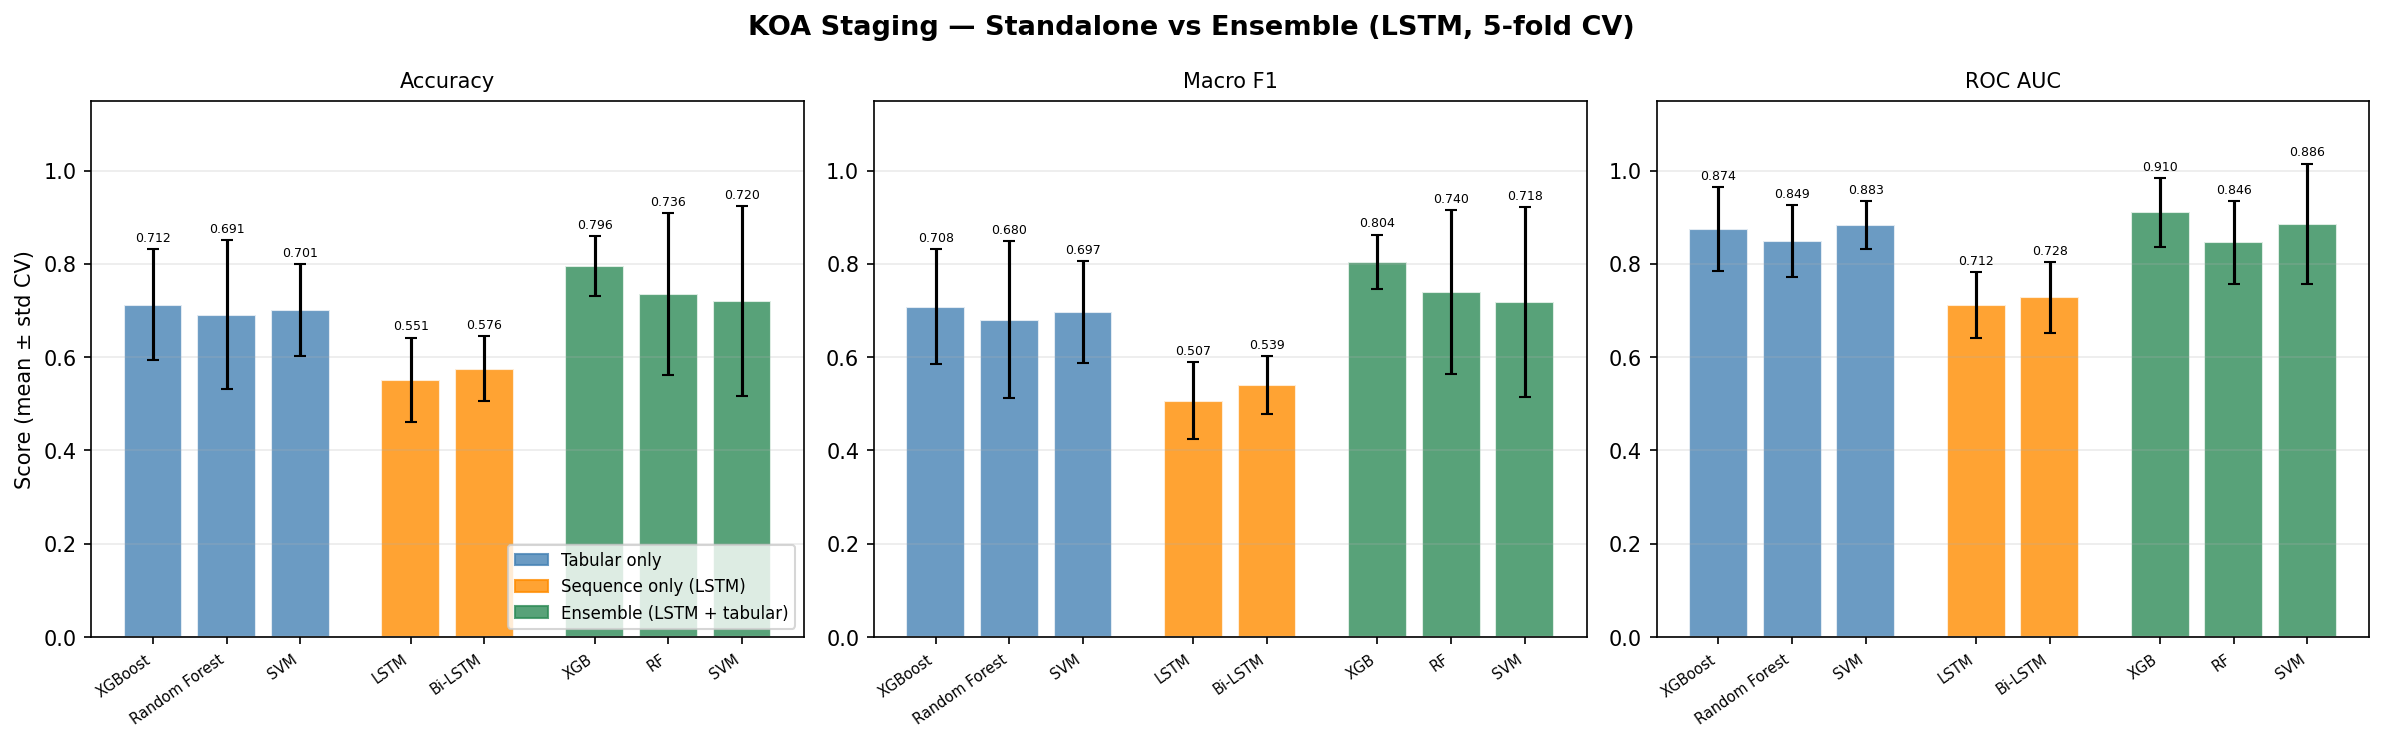
\includegraphics[width=0.85\textwidth]{ensemble_comparison_koastage.png}
  \caption{Comparação de desempenho dos modelos ensemble na Tarefa~B
           (estadiamento KOA). Barras representam média $\pm$ desvio padrão entre
           5 \textit{folds}.}
  \label{fig:ensemble_b}
\end{figure}

\begin{figure}[H]
  \centering
  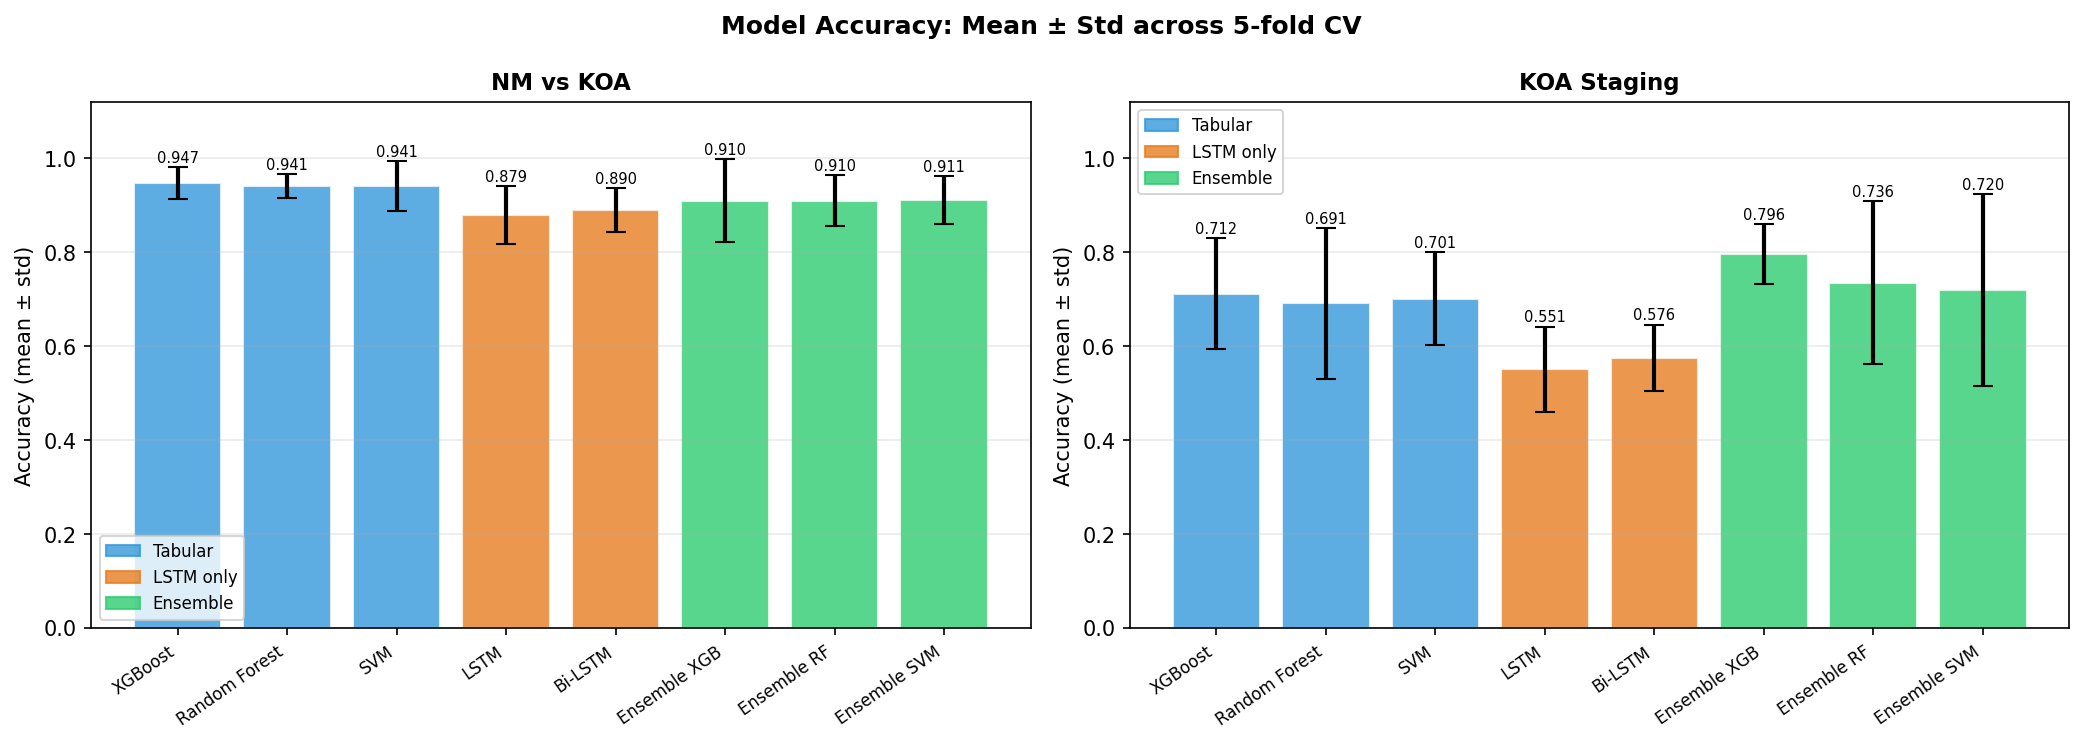
\includegraphics[width=0.85\textwidth]{all_models_accuracy_cv.png}
  \caption{Acurácia de todos os modelos em ambas as tarefas (validação cruzada).}
  \label{fig:all_models}
\end{figure}

\subsection{Importância de \textit{Features}}

A importância média das \textit{features} do XGBoost (ganho de informação, média
entre \textit{folds}) revela os parâmetros biomecânicos mais discriminativos
(Tabela~\ref{tab:fimp}).

\begin{table}[H]
  \centering
  \caption{Top-5 \textit{features} por importância XGBoost (média entre
           \textit{folds}).}
  \label{tab:fimp}
  \begin{tabular}{@{}cll@{}}
    \toprule
    \textbf{Rank} &
    \textbf{Tarefa~A --- NM vs.\ KOA} &
    \textbf{Tarefa~B --- KOA Staging} \\
    \midrule
    1 & Comprimento médio de passo (px) & Comprimento médio de passo (px) \\
    2 & Tempo de apoio esquerdo (s)     & ROM joelho direito (°) \\
    3 & CV ciclo joelho esquerdo (\%)   & Tempo médio de passo (s) \\
    4 & ROM joelho esquerdo (°)         & ROM joelho esquerdo (°) \\
    5 & Mínimo joelho esquerdo (°)      & Qualidade média (\%) \\
    \bottomrule
  \end{tabular}
\end{table}

O comprimento de passo é a \textit{feature} de maior poder discriminativo em ambas
as tarefas, seguida por parâmetros cinemáticos do joelho. Isso é consistente com a
fisiopatologia: pacientes com KOA encurtam o comprimento de passo para reduzir o
estresse articular~\cite{Stenum2021}, e a ROM do joelho diminui progressivamente com
o avanço da doença.

A análise da contribuição por modalidade no ensemble (importância de ganho do
XGBoost):
\begin{itemize}
  \item \textbf{Tarefa A}: \textit{features} tabulares = 96,5\%;
        \textit{embeddings} LSTM = 3,5\%.
  \item \textbf{Tarefa B}: \textit{features} tabulares = 99,2\%;
        \textit{embeddings} LSTM = 0,8\%.
\end{itemize}

Embora a importância de ganho dos \textit{embeddings} LSTM seja baixa, eles
contribuem para \textit{splits} que resolvem casos limítrofes não discriminados pelas
\textit{features} tabulares, resultando no ganho observado de +8,4~pp na Tarefa~B.

\subsection{Ablação do Encoder: LSTM vs.\ Bi-LSTM}

A Tabela~\ref{tab:ablation} compara o desempenho dos modelos ensemble com encoder
LSTM unidirecional e bidirecional sob os mesmos hiperparâmetros, \textit{seed} e
\textit{folds}.

\begin{table}[H]
  \centering
  \caption{Ablação do encoder: LSTM (dim~=~64) vs.\ Bi-LSTM (dim~=~128).}
  \label{tab:ablation}
  \begin{tabular}{@{}llcccc@{}}
    \toprule
    \textbf{Tarefa} & \textbf{Encoder} &
    \textbf{Acurácia} & \textbf{F1 Macro} & \textbf{AUC} &
    \textbf{Dim.\ vetor} \\
    \midrule
    NM vs.\ KOA  & LSTM    & 0,910 $\pm$ 0,088 & 0,904 $\pm$ 0,093 & 0,972 & 115 \\
    NM vs.\ KOA  & Bi-LSTM & 0,901 $\pm$ 0,082 & 0,896 $\pm$ 0,091 & 0,969 & 179 \\
    KOA Staging  & \textbf{LSTM}
                 & \textbf{0,796 $\pm$ 0,064}
                 & \textbf{0,804 $\pm$ 0,059} & 0,911 & 115 \\
    KOA Staging  & Bi-LSTM & 0,780 $\pm$ 0,091 & 0,779 $\pm$ 0,095
                 & \textbf{0,916} & 179 \\
    \bottomrule
  \end{tabular}
\end{table}

O encoder LSTM unidirecional iguala ou supera o Bi-LSTM em ambas as tarefas, com um
vetor de \textit{embedding} de metade da dimensionalidade (64 vs.\ 128 dimensões;
vetor combinado: 115 vs.\ 179). Na Tarefa~B, o LSTM supera o Bi-LSTM em
+1,6~pp de acurácia (+2,5~pp de F1 macro), sugerindo que o contexto futuro
fornecido pelo processamento reverso do Bi-LSTM não acrescenta informação relevante
para este problema, possivelmente porque as \textit{features} tabulares já capturam
os padrões globais do ciclo.

% ============================================================
\section{Discussão}
\label{sec:disc}
% ============================================================

\subsection{Por que o XGBoost Tabular é Suficiente para a Tarefa~A}

As \textit{features} espaço-temporais --- especialmente o comprimento de passo e os
parâmetros de apoio --- apresentam alta separabilidade entre NM e KOA. Pacientes com
KOA encurtam o comprimento de passo (redução média de $\approx$81 pixels,
equivalente a $\approx$58\% de diferença) e prolongam o tempo de apoio como
estratégia compensatória para reduzir o pico de carga articular. Esses parâmetros
agregados são captados integralmente pelas \textit{features} tabulares, deixando
pouca margem para que o \textit{embedding} LSTM contribua adicionalmente. Esse
padrão justifica a ausência de ganho do ensemble na Tarefa~A.

\subsection{Por que o Ensemble Melhora o Estadiamento (Tarefa~B)}

A distinção entre os três estágios de KOA --- especialmente entre precoce (EL) e
moderado (MD) --- não é completamente capturada pelas \textit{features} tabulares
globais. O ROM do joelho diminui monotonicamente com a severidade
(EL: $\approx$46°, MD: $\approx$40°, SV: $\approx$33°), mas apresenta
\textit{overlap} considerável entre grupos adjacentes. O \textit{embedding} LSTM
retém informações sobre o padrão temporal do ângulo ao longo do ciclo --- como a
posição do pico e a velocidade angular nas fases de carga e balanço --- que não estão
representadas nas estatísticas de primeiro e segundo momentos das \textit{features}
tabulares. Essa informação complementar, ainda que de baixa importância de ganho
individual (0,8\%), contribui para resolução de casos limítrofes, resultando em
+8,4~pp de acurácia.

\subsection{Posicionamento em Relação à Literatura}

Este trabalho obtém o \textbf{melhor resultado reportado em estadiamento de KOA sob
protocolo de validação a nível de sujeito} (79,6\% vs.\ 76,6\% de Kaya et
al.~\cite{Kaya2025}), utilizando um pipeline computacionalmente mais acessível:
OpenPose 2D em vez de AlphaPose + HybrIK 3D, e \textit{features} biomecânicas
interpretáveis em vez de sequências de 24 \textit{keypoints} 3D por \textit{frame}.

A comparação direta com o trabalho de Kaya et al.~\cite{Kaya2025} é particularmente
relevante porque é o único outro estudo que adota validação por sujeito e relata
resultados tanto para classificação binária quanto para estadiamento no mesmo dataset.
Kaya et al.\ reportam queda de 14~pp ao migrar de \textit{random split} (90,8\%) para
\textit{subject split} (76,6\%), evidenciando o efeito do \textit{data leakage}.
Este trabalho opera exclusivamente sob protocolo a nível de sujeito, sem comparação
com \textit{random split}.

Ben Hassine et al.~\cite{BenHassine2024} reportam 96,9\% na classificação binária
NM vs.\ KOA, levemente acima dos 94,7\% deste trabalho, porém o protocolo de
validação não é detalhado no artigo --- impossibilitando confirmar se a comparação é
justa.

\subsection{Limitações}

\textbf{Estimativa de pose 2D vs.\ 3D:} O OpenPose Body25 opera no plano sagital e
não captura movimentos nos planos frontal e transverso (adução/abdução do joelho,
rotação), que são clinicamente relevantes para KOA. A alta variância do ROM do
quadril ($\sigma \approx 23°$), comparado ao joelho ($\sigma \approx 9°$), é
consistente com essa limitação: movimentos do quadril fora do plano sagital
introduzem ruído nas estimativas 2D.

\textbf{Comprimento de passo em pixels:} A \textit{feature} de maior importância
discriminativa não é calibrada em unidades métricas, introduzindo potencial
confundidor de estatura entre sujeitos. Normalização pelo comprimento do membro
inferior (estimado pela distância quadril--tornozelo nos \textit{keypoints}) poderia
reduzir essa variância.

\textbf{N amostral pequeno e alta variância entre \textit{folds}:} Com
$\approx$10 sujeitos por \textit{fold} na Tarefa~B, a estimativa de desempenho por
\textit{fold} apresenta variância elevada (desvio padrão de 6--16\%). Essa limitação
é inerente ao dataset e afeta igualmente todos os trabalhos comparados.

\textbf{Grupo PD não incluído:} O dataset de Kour et al.~\cite{Kour2022} inclui 16
participantes com doença de Parkinson, cujos padrões de marcha diferem tanto de NM
quanto de KOA. A classificação tripartite NM/KOA/PD é uma extensão natural deste
trabalho.

\textbf{Generalização demográfica:} O dataset foi coletado em ambiente clínico na
Índia, com sujeitos de estatura média $\approx$1,56~m. A generalização para
populações com diferentes distribuições antropométricas não foi avaliada.

% ============================================================
\section{Conclusão}
% ============================================================

Este trabalho apresentou um pipeline completo e auditável para classificação
automática de KOA a partir de vídeos sagitais de marcha 2D. As principais conclusões
são:

\begin{enumerate}[label=\arabic*.]
  \item \textbf{\textit{Features} biomecânicas tabulares são suficientes para
        triagem NM vs.\ KOA:} XGBoost tabular atinge 94,7\% de acurácia e
        AUC~=~0,994 com validação a nível de sujeito, demonstrando que parâmetros
        como comprimento de passo, ROM do joelho e tempo de apoio são altamente
        discriminativos.

  \item \textbf{O ensemble LSTM+tabular é necessário para o estadiamento de
        severidade:} O ensemble XGB com encoder LSTM atinge 79,6\% de acurácia no
        estadiamento EL/MD/SV (+8,4~pp sobre XGBoost tabular), evidenciando que a
        informação temporal do ciclo complementa os parâmetros agregados.

  \item \textbf{Validação a nível de sujeito é determinante:} O protocolo
        \texttt{StratifiedGroupKFold} por sujeito produz estimativas mais
        conservadoras e realistas do que o \textit{random split}, consistente com
        os achados de Kaya et al.~\cite{Kaya2025}.

  \item \textbf{LSTM unidirecional iguala ou supera o Bi-LSTM} com metade da
        dimensionalidade de \textit{embedding}, recomendando-se o LSTM como encoder
        de menor complexidade para este domínio.

  \item \textbf{Pipeline acessível e interpretável:} OpenPose Body25 em câmera 2D
        monocular, sem marcadores ou sensores especializados, com \textit{features}
        biomecânicas de significado clínico direto.
\end{enumerate}

\noindent\textbf{Trabalho futuro} inclui: (i) inclusão do grupo PD para
classificação tripartite; (ii) calibração métrica do comprimento de passo por
comprimento de membro estimado via \textit{keypoints}; (iii) análise SHAP para
interpretabilidade a nível de ciclo individual; e (iv) validação em coorte
independente.

% ============================================================
\bibliographystyle{unsrtnat}
\bibliography{references}
% ============================================================

\end{document}
